\documentclass[tikz,border=4pt]{standalone}
\usepackage{amsmath,amssymb}
\usetikzlibrary{arrows.meta}

\begin{document}
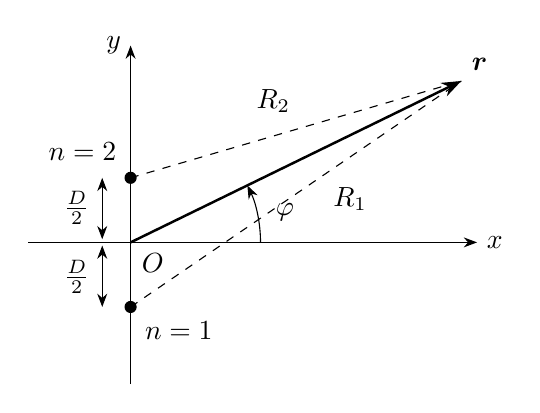
\begin{tikzpicture}[
  >=Stealth,
  font=\normalsize,
  axis/.style={line width=0.4pt},
  curve/.style={line width=0.9pt}
]
  % Axes
  \draw[axis,->] (-1.3,0) -- (4.4,0) node[right] {$x$};
  \draw[axis,->] (0,-1.8) -- (0,2.5) node[left] {$y$};
  \node[below right] at (0.02,-0.02) {$O$};

  % Two sources at (0, -0.82) and (0, +0.82)
  \fill (0,-0.82) circle (2.2pt);
  \fill (0,0.82) circle (2.2pt);
  \node[below right] at (0.06,-0.88) {$n = 1$};
  \node[above left] at (-0.06,0.92) {$n = 2$};

  % D/2 dimensions
  \draw[axis,<->] (-0.36,0.04) -- (-0.36,0.82);
  \node[left] at (-0.40,0.44) {$\tfrac{D}{2}$};
  \draw[axis,<->] (-0.36,-0.82) -- (-0.36,-0.04);
  \node[left] at (-0.40,-0.44) {$\tfrac{D}{2}$};

  % Observation point r
  \coordinate (P) at (4.2,2.05);
  \draw[curve,->] (0,0) -- (P) node[above right] {$\boldsymbol{r}$};
  \draw[axis,dashed] (0,-0.82) -- (P);
  \draw[axis,dashed] (0,0.82) -- (P);

  % Labels R_1, R_2
  \node[below right] at (2.45,0.82) {$R_1$};
  \node[above left] at (2.15,1.52) {$R_2$};

  % Angle phi
  \draw[axis,->] (1.65,0) arc (0:26:1.65);
  \node[right] at (1.72,0.38) {$\varphi$};
\end{tikzpicture}
\end{document}
